\chapter{Developing for CxAnalytix}

\section{Build From Source}

\subsection{The Easy Way}
The easiest method of building the code from source is to open the \texttt{CxAnalytix.sln} file using Visual Studio (not Visual Studio Code).
From there, the entire solution can be built with a "Build Solution" command.

\subsection{From the Command Line}
If the .Net Core SDK of the appropriate version is installed, the \texttt{dotnet} command can be executed to create a build:\\

\begin{code}{Build Commands}{}{}
dotnet publish .\CxAnalytix.sln -o $OutLoc/win-x64 -c ReleaseWindows -r win-x64
dotnet publish .\CxAnalytix.sln -o $OutLoc/linux-x64 -c ReleaseLinux -r linux-x64
\end{code}

\subsection{Visual Studio Code}
This is a .Net Core application and therefore can be developed on any platform that supports .Net Core.  Readers are encouraged to investigate configuring
their instance of VSCode to build and debug CxAnalytix.  A basic \texttt{launch.json} and \texttt{tasks.json} file is included in the source tree, but they may need
updated as versions of .Net Core and VSCode change over time.


\subsection{GitHub Workflows}

The GitHub workflows are part of the official CxAnalytix repository that are used to build and publish release and pre-release builds.  Forks of the CxAnalytix
repository can also use these workflows to build and publish release artifacts.\footnote{GitHub will, by default, disable the workflows on forks.  You will need token
visit the \texttt{Actions} tab of your repository to enable the workflows.}

\noindent\\By default, the \texttt{build-ci} workflow executes on pushes, pull requests, or pull request updates on any branch.  The CI build is meant to
assure that code changes have not broken the build process.  No artifacts are published as part of the CI build.

\noindent\\The \texttt{build-release} and \texttt{build-prerelease} workflows are used to publish release and pre-release artifacts.  Platform specific zip and pdf 
artifacts are published in the code Releases section of GitHub.  A Docker image is also published in the owning organization's GitHub packages repository as 
\\\texttt{cxanalytix/cxanalytix:\textit{<tag>}}.  Each workflow requires the following Action secrets to be defined:

\begin{table}[h]
    \caption{GitHub Action Secrets}        
    \begin{tabularx}{\textwidth}{ll}
        \toprule
        \textbf{Secret Name} & \textbf{Description} \\
        \midrule
        \texttt{PACKAGE\_PAT} & \makecell[l]{A personal access token that has the appropriate permissions\\to perform build operations.} \\
        \midrule
        \texttt{PACKAGE\_USER} & The user associated with the PAT. \\
        \bottomrule
    \end{tabularx}
\end{table}

\noindent\\The package PAT requires the permissions that allow the following build operations:\\

\begin{enumerate}
    \item Set and delete tags on the CxAnalytix repository.
    \item Publish releases for the CxAnalytix repository.
    \item Publish packages in the CxAnalytix repository's owning organization.
\end{enumerate}

\subsubsection{Invoking the GitHub Release and Pre-Release Workflows}

\noindent\\The \texttt{build-release} and \texttt{build-prerelease} workflows are typically manually invoked by navigating to \texttt{Actions}
and highlighting the workflow that is to be invoked.  The \texttt{Run Workflow} button on the right side of the screen, as shown in the screen
shot below, allows a branch to be chosen and a release version to be defined.  If everything executes correctly, a release or pre-release
is published and the repository is tagged.

\noindent\\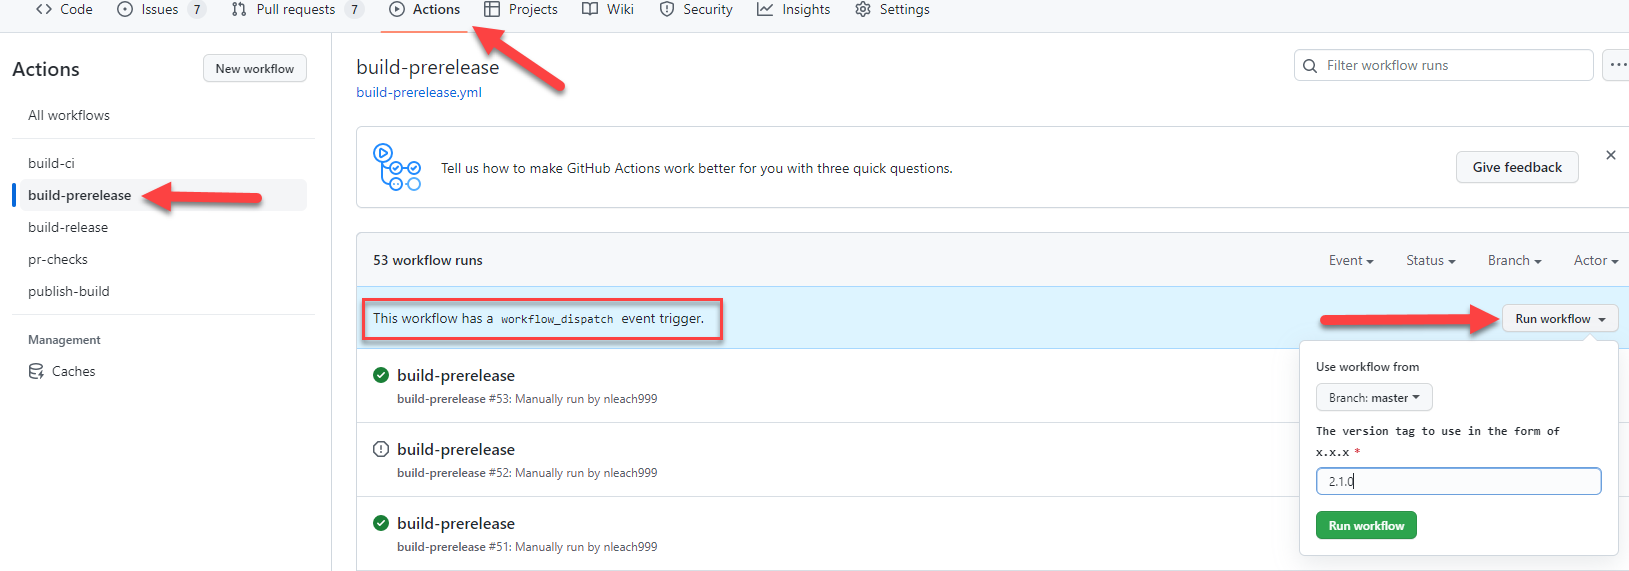
\includegraphics[scale=.4]{graphics/github-workflow.png}

\section{Developing New Modules}

The transformation and output modules are dynamically loaded at runtime.  They are developed with an SDK component included in the CxAnalytix source tree.
The SDK component is intended to be used as a project reference at this time as it is not deployed as a Nuget package.

\noindent\\The modules, being that they are dynamically loaded, will have no incoming dependencies.  This means they will not be included
in the build output since the compiler will believe the shared libraries where the modules are implemented are not in use.  For easy debug and build
purposes, each output and transform module is added as a project dependency to the \texttt{Executive} project.  The \texttt{Executive} project
is loaded by executing applications on all platforms to perform the appropriate type of CxAnalytix execution.


\subsection{Creating New Transformation Modules}

Creating a new transformer type can be done with the following steps:

\begin{enumerate}
    \item Create a class library project.
    \item Add a project reference to \texttt{SDK.Modules}
    \item Create a class that derives from \texttt{TransformerModule}
    \item Create a public default constructor that initializes the transformer module with the runtime specifics of your module
    \item Implement the abstract methods/properties defined in \texttt{TransformerModule}
\end{enumerate}

\noindent\\An example transformer module can be observed in the code snippet \hyperref[lst:xform]{Example Transformer Module}. The arguments passed to 
the \texttt{TransformerModule} are explained in table \ref{tab:xform}.\\


\begin{table}
    \centering
    \begin{tabular}{|c|c|l|}
        \toprule
        \textbf{Argument} & \textbf{Type} & \textbf{Description}\\
        \midrule
        \texttt{moduleName} & \texttt{String} & \makecell[l]{The string used to select the module for invocation in the\\
        configuration as described in section \ref{sec:general} (e.g. SAST, SCA)}\\
        \midrule
        \texttt{moduleImplType} & \texttt{Type} & The .Net type that contains the implementation of the module.\\
        \midrule
        \texttt{stateStorageFileName} & \texttt{String} & The name of the file that stores any state of the transformation module.\\
        \bottomrule
    \end{tabular}
    \caption{\texttt{TransformerModule} Construction Parameters}
    \label{tab:xform}
\end{table}



\begin{code}{Example Transformer Module}{\label{lst:xform}}{}
class Transformer : TransformerModule
{
    public override string DisplayName 
        => "This is my module, this text will show in logs";

    
    public Transformer() 
        : base("MYMODULE", typeof(Transformer), "MYMODULE_state.json")
    {
        // Initialization goes here, if any
    }

    public override void DoTransform(CancellationToken token)
    {
        // This is where the transformation is executed.
    }
}
\end{code}

\subsection{Creating New Output Modules}

Output modules are created similarly to transformer modules.  The basic tasks to create an output module:

\begin{enumerate}
    \item Create a class library project.
    \item Add a project reference to \texttt{SDK.Modules}
    \item Create a class that derives from \texttt{OutputModule}; this is your factory class that creates the instance of the output implementation
    \item Create a public default constructor that initializes the output module with the runtime specifics of your module
    \item Implement the abstract methods/properties defined in \texttt{OutputModule}
\end{enumerate}

\noindent\\The snippet \hyperref[lst:output]{Example Output Module} shows an example of an output implementation.  Table \ref{tab:output} explains the output
module arguments.


\begin{code}{Example Output Module}{\label{lst:output}}{}
public class MyOutFactory : SDK.Modules.Output.OutputModule
{
    public MyOutFactory() : base("MyOutput", typeof(MyOutFactory) )
    {
    }

    public override IRecordRef RegisterRecord(string recordName)
    {
        // Implementation for registering a record
    }

    public override IOutputTransaction StartTransaction()
    {
        // This is where the instance of the output implementation is given
        // to the caller.  Transactional capabilities are optional, the
        // concept of a transaction is simply a grouping of related
        // data being output.
    }
}    
\end{code}


\begin{table}
    \centering
    \begin{tabular}{|c|c|l|}
        \toprule
        \textbf{Argument} & \textbf{Type} & \textbf{Description}\\
        \midrule
        \texttt{moduleName} & \texttt{String} & \makecell[l]{The string used to select the module for output in the\\
        configuration as described in section \ref{sec:general} (e.g. MongoDB, AMQP, Log4Net)}\\
        \midrule
        \texttt{moduleImplType} & \texttt{Type} & The .Net type that contains the implementation of the module.\\
        \bottomrule
    \end{tabular}
    \caption{\texttt{OutputModule} Construction Parameters}
    \label{tab:output}
\end{table}


\section{Module Configuration}

\subsection{CxAnalytix Internal Configuration}\label{sec:internal_config}

It is possible to obtain the general configuration objects (described in section \ref{sec:general}) with a project dependency for the \texttt{Configuration}
class library.  Obtaining a reference to the \texttt{CxAnalytixService} configuration can then be achieved with the example code show in the 
\hyperref[lst:global_config]{code snippet below}.  Instances of CxAnalytix configuration objects can be obtained by specifying the type in the generic parameter for the 
method call \texttt{CxAnalytix.Configuration.Impls.Config.GetConfig<T>()} 


\begin{code}{Retrieving a CxAnalytixService Config Object Instance}{\label{lst:global_config}}{}
private CxAnalytixService Service => 
    CxAnalytix.Configuration.Impls.Config.GetConfig<CxAnalytixService>();
\end{code}


\subsection{Module-Specific Configuration}

All configurations in the \texttt{cxanalytix.config} file are consumed by the Microsoft\\ 
\texttt{System.Configuration.ConfigurationManager} package.
Each individual module implementation should define configuration classes that are publicly accessible for dynamic loading.
The assembly path for custom module configuration is then placed in the \texttt{configSections} element of the \texttt{cxanalytix.config}
file.  The \hyperref[lst:config_sections]{AMQP Configuration Section Entries} snippet shows an example of a configuration section entry to load the AMQP configuration elements
from the AMQP class library.

\noindent\\Obtaining an instance of a configuration object uses the same \texttt{GetConfig} as was used in section \ref{sec:internal_config}
to obtain an instance of the \texttt{CxAnalytixService} configuration object.  The \hyperref[lst:amqp_config]{Retrieving a Config Object Instance} snippet 
shows an example of how the AMQP output module obtains an instance of an module-specific configuration object.\\

\begin{code}{AMQP Configuration Section Entries}{\label{lst:config_sections}}{}
<configSections>
    <section name="AMQPConnection" 
        type="CxAnalytix.Out.AMQPOutput.Config.Impls.AmqpConnectionConfig, AMQPOutput"
        />
    <section name="AMQPConfig" 
        type="CxAnalytix.Out.AMQPOutput.Config.Impls.AmqpConfig, AMQPOutput"
        />
</configSections>
\end{code}


\begin{code}{Retrieving a Config Object Instance}{\label{lst:amqp_config}}{}
private AmqpConnectionConfig ConConfig =>
    CxAnalytix.Configuration.Impls.Config.GetConfig<AmqpConnectionConfig>();
\end{code}
    